\documentclass{standalone}
\usepackage{picture,color}
\usepackage{graphicx}
\graphicspath{{./Fig_PFC_subfigs/}}
\setlength{\unitlength}{1in}
\usepackage{helvet}
\renewcommand{\familydefault}{\sfdefault}
\begin{document}
\begin{picture}(6.85, 6.55)(0,-6.8)
% example frame 
\put(0.15, -1.4){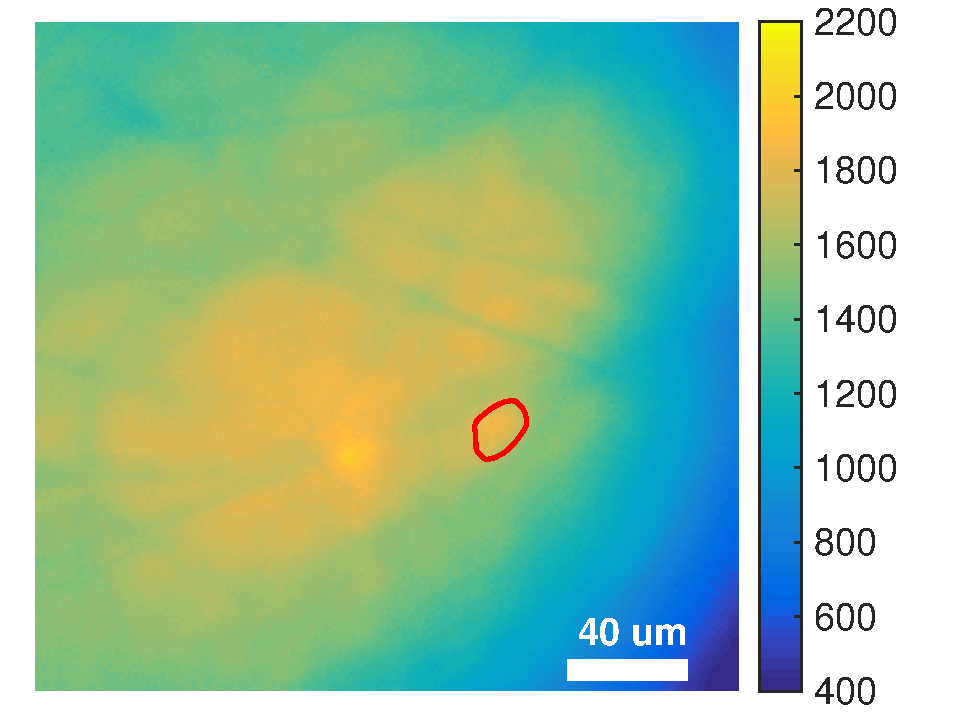
\includegraphics[height=1in]{Fig_PFC_subfigs/example_frame.pdf}}
\put(0.02, -0.45){\large\textbf{A}}
\put(.48, -0.4){\scriptsize Raw data}

\put(1.41,-0.95){\large\textbf{=}}
\put(1.50, -1.4){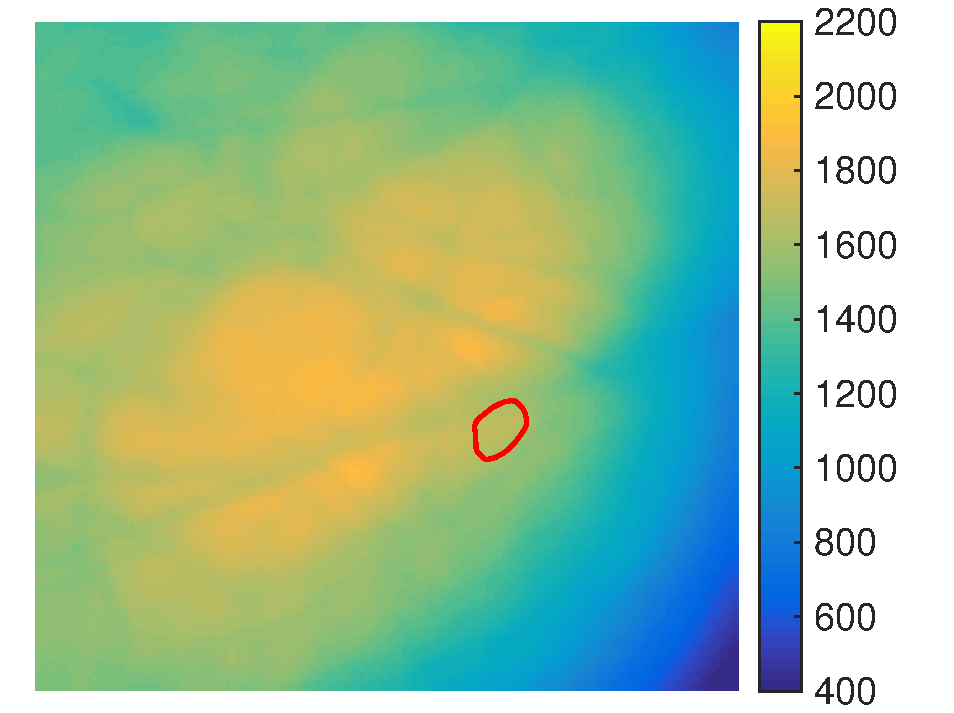
\includegraphics[height=1in]{Fig_PFC_subfigs/example_frame_bg_constant.pdf}}
\put(1.7, -0.4){\scriptsize Const. baseline}

\put(2.76,-0.95){\large\textbf{+}}
\put(2.85, -1.4){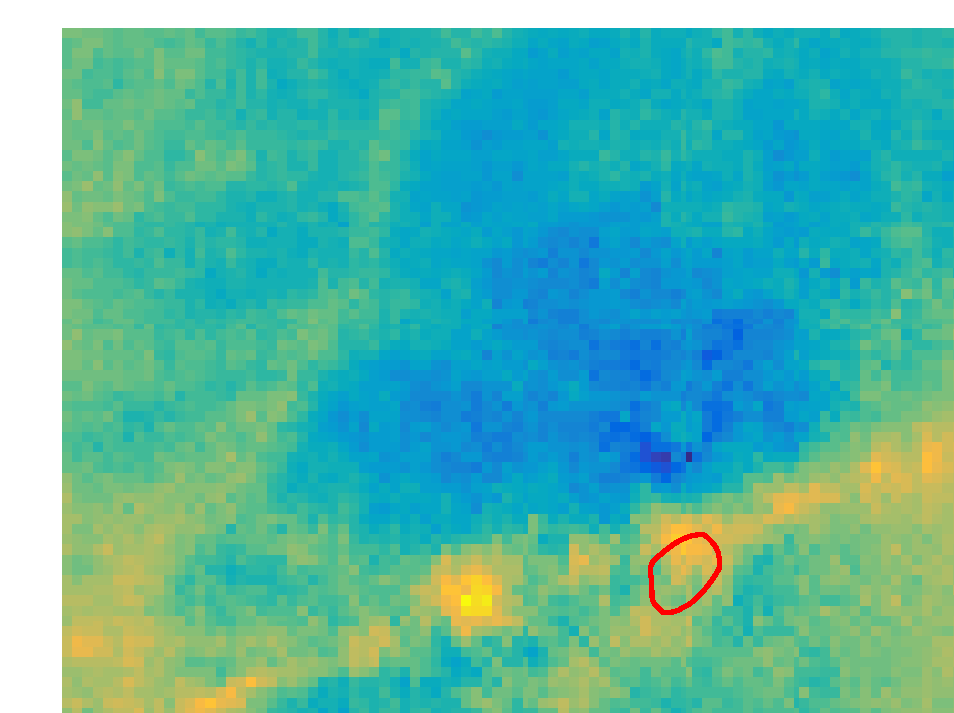
\includegraphics[height=1in]{Fig_PFC_subfigs/example_frame_bg_fluc.pdf}}
\put(3.03, -0.4){\scriptsize Fluc. background}

\put(4.11,-0.95){\large\textbf{+}}
\put(4.2, -1.4){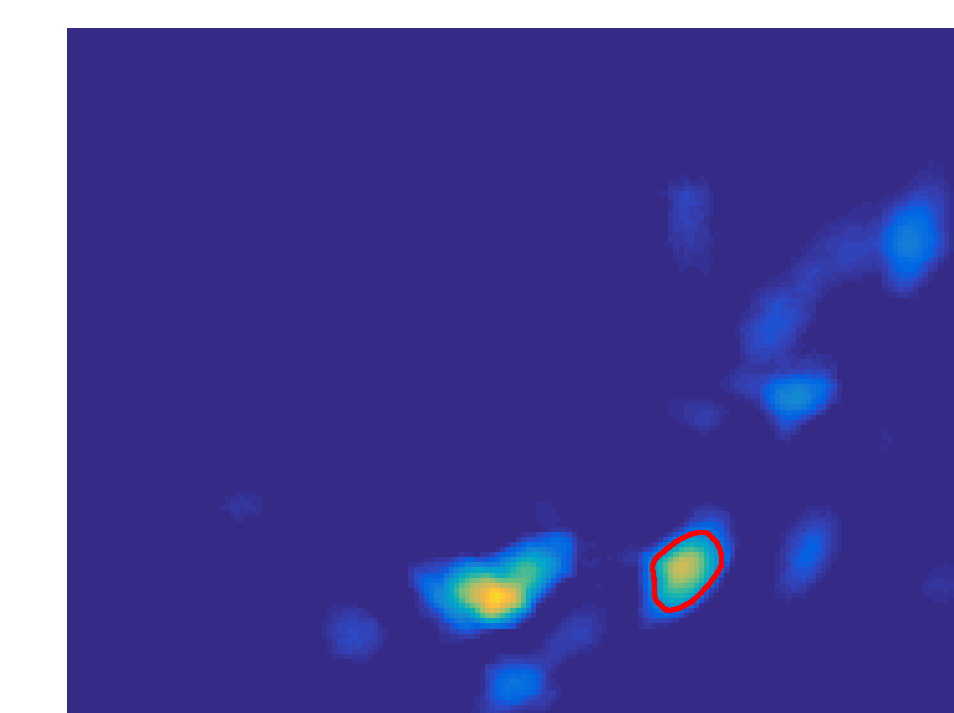
\includegraphics[height=1in]{Fig_PFC_subfigs/example_frame_ac.pdf}}
\put(4.46, -0.4){\scriptsize Neural signal}

\put(5.46,-0.95){\large\textbf{+}}
\put(5.55, -1.4){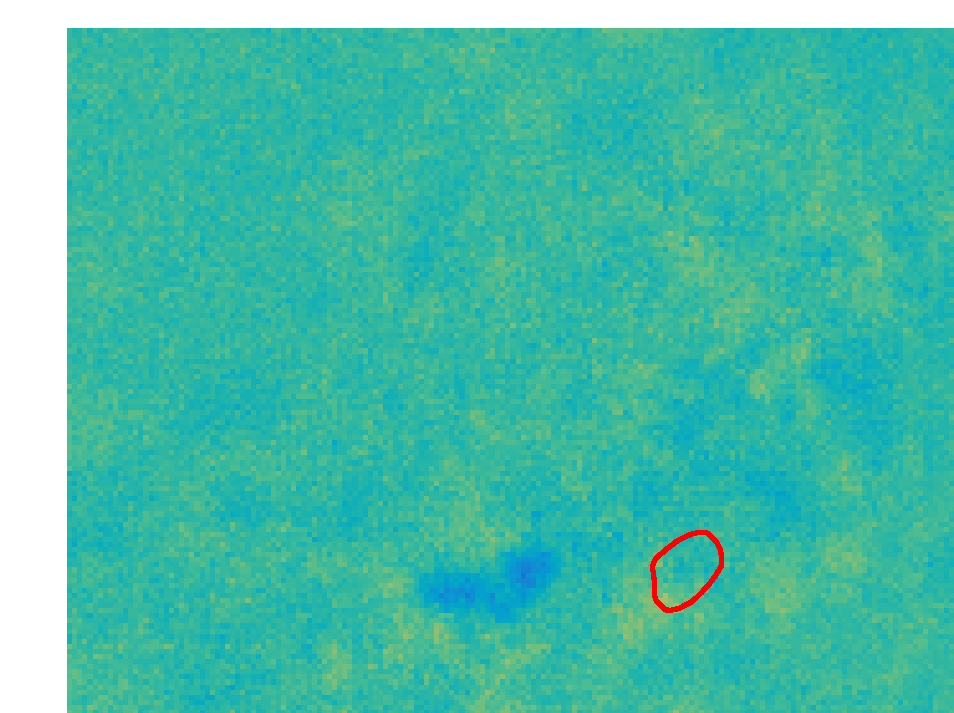
\includegraphics[height=1in]{Fig_PFC_subfigs/example_frame_res.pdf}}
\put(5.89, -0.4){\scriptsize Residual}

% % traces within an selected ROI 
% \put(0.08, -3.0){\includegraphics[height=1.43in]{Fig_PFC_subfigs/example_roi_traces.pdf}}
% \put(0.02, -1.59){\large\textbf{B}}
% \put(0.55, -1.53){\scriptsize Fluorescence traces within the ROI}
% explained variance 
\put(0.08, -3.15){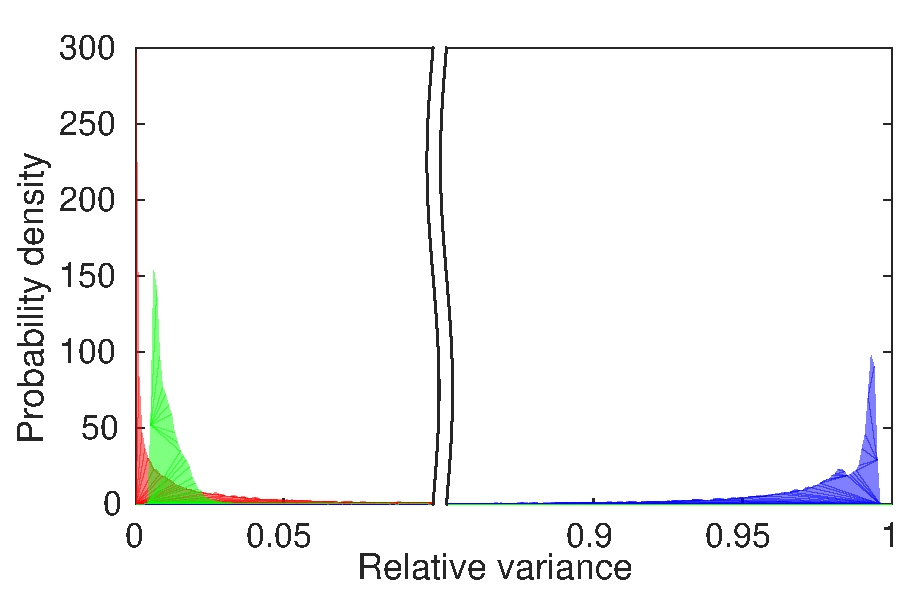
\includegraphics[height=1.65in]{Fig_PFC_subfigs/variance_explained.pdf}}
\put(0.02, -1.59){\large\textbf{B}}
\put(1.0, -1.55){\scriptsize Explained Variance}

% explained variance 
% \put(2.28, -3.00){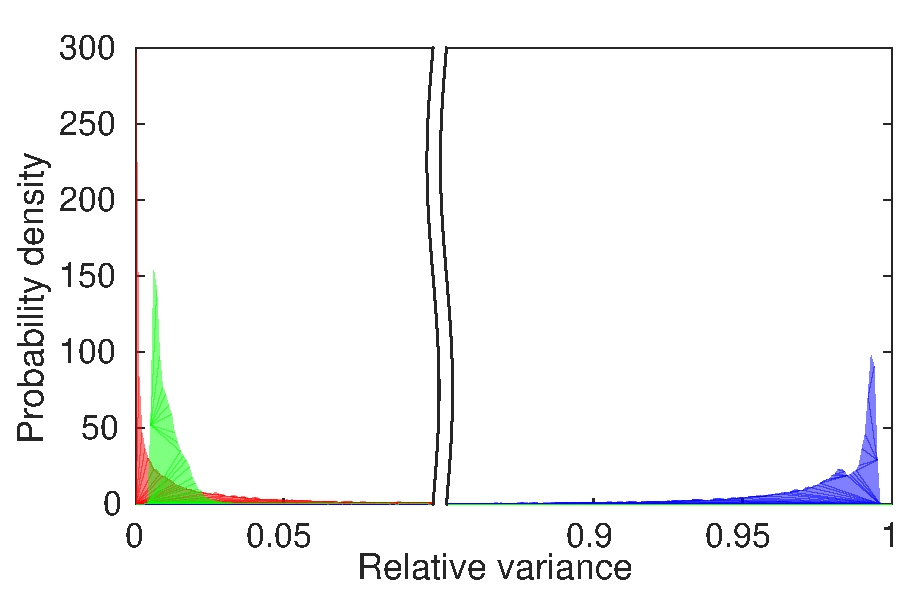
\includegraphics[height=1.5in]{Fig_PFC_subfigs/variance_explained.pdf}}
% \put(2.26, -1.59){\large\textbf{C}}
% \put(3.15, -1.53){\scriptsize Explained Variance}

% contour plot  
\put(4.85, -3.15){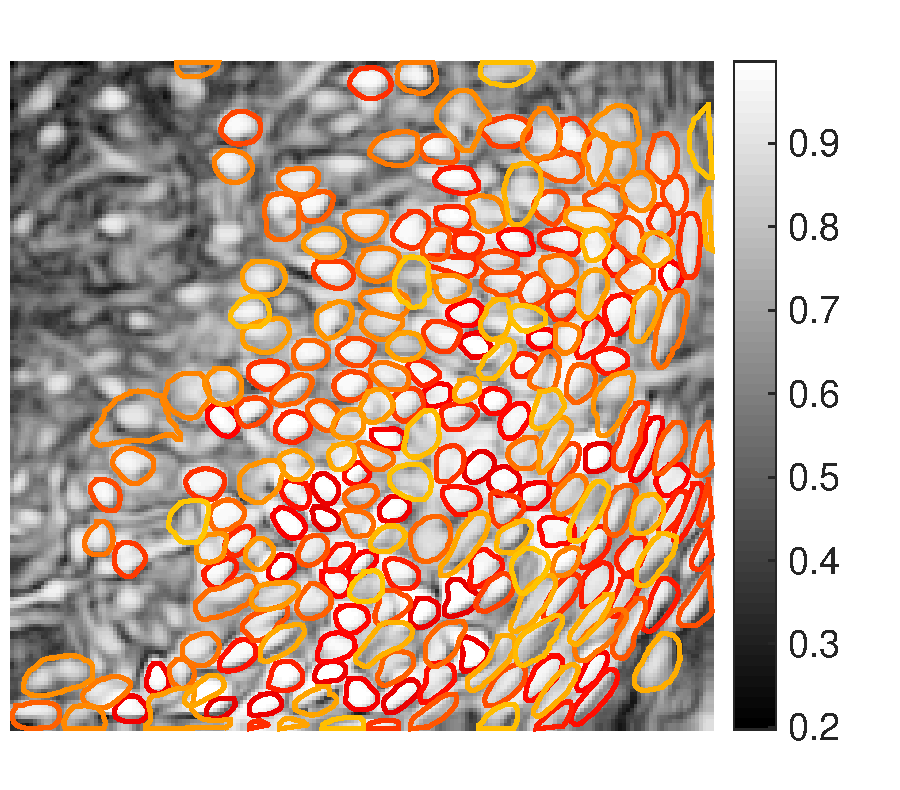
\includegraphics[height=1.7in]{Fig_PFC_subfigs/contours_ica.pdf}}
\put(2.85, -3.15){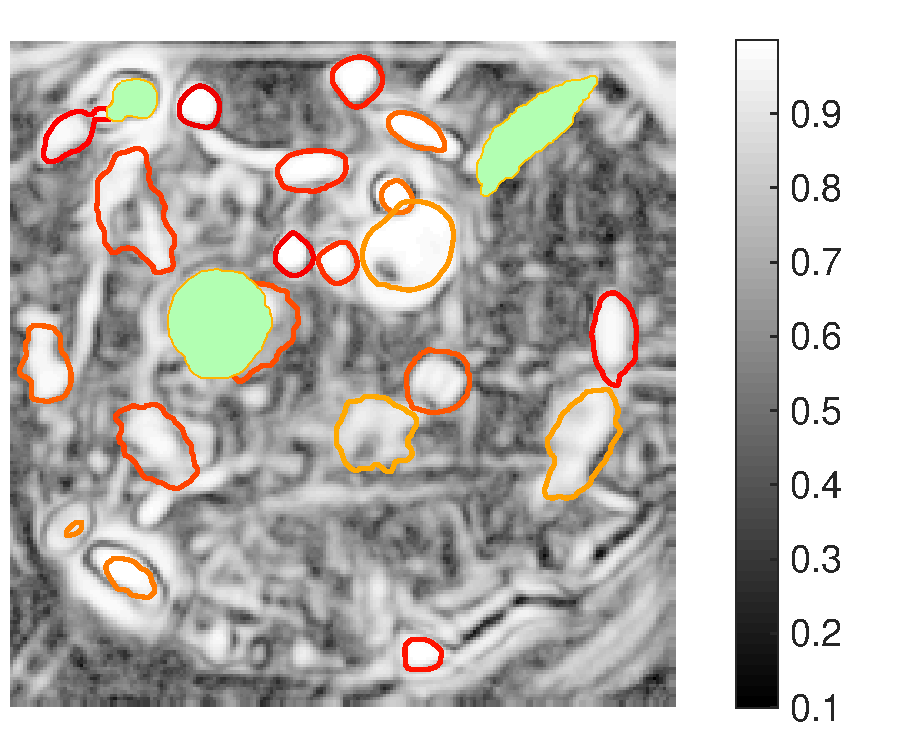
\includegraphics[height=1.7in]{Fig_PFC_subfigs/contours_cnmfe.pdf}}
\put(2.7, -1.59){\large\textbf{C}}
\put(3.5, -1.55){\scriptsize CNMF-E}
\put(5.5, -1.55){\scriptsize PCA/ICA}

% \put(5.5, -1.53){\scriptsize Contour plot}
% \put(4.72, -1.59){\line(1,0){2.08}}
% \put(6.8,-1.59){\line(0, -1){3.2}}
% \put(4.72, -1.59){\line(0,-1){3.2}}
% \put(4.72, -4.79){\line(1,0){2.08}}
% \put(4.77, -2.7){\rotatebox{90}{CNMF-E}}
% \put(4.77, -4.3){\rotatebox{90}{PCA/ICA}}

\put(0.08, -5.05){\includegraphics[height=1.73in]{Fig_PFC_subfigs/snr_pca_ica.pdf}}
\put(0.02, -3.33){\large\textbf{D}}
\put(0.68, -3.28){\scriptsize SNR}

% matched neurons 
\put(2.22, -5.05){\includegraphics[height=0.6in]{Fig_PFC_subfigs/colorbar_ica.pdf}}
\put(1.57, -5.05){\includegraphics[height=0.6in]{Fig_PFC_subfigs/colorbar_cnmfe.pdf}}
\put(1.58, -4.8){\includegraphics[height=1.45in]{Fig_PFC_subfigs/match_spatial_cnmfe.pdf}}
\put(2.23, -4.8){\includegraphics[height=1.45in]{Fig_PFC_subfigs/match_spatial_ICA.pdf}}
\put(1.42, -3.33){\large\textbf{E}}
\put(1.66, -3.28){\scriptsize CNMF-E}
\put(2.31, -3.28){\scriptsize PCA/ICA}
\put(4.70, -5.0){\includegraphics[height=1.75in]{Fig_PFC_subfigs/matched_temporal_ica.pdf}}
\put(2.8, -5.0){\includegraphics[height=1.75in]{Fig_PFC_subfigs/matched_temporal_cnmfe.pdf}}
\put(3.5, -3.28){\scriptsize CNMF-E traces}
\put(5.35, -3.28){\scriptsize PCA/ICA traces}

\put(0.18, -5.52){\includegraphics[height=0.28in]{Fig_PFC_subfigs/ica_missed_spatial.pdf}}
\put(0.01, -6.75){\includegraphics[height=1.2in]{Fig_PFC_subfigs/ica_missed_temporal.pdf}}
\put(0.02, -5.23){\large\textbf{F}}
\put(0.8, -5.18){\scriptsize Components detected by CNMF-E only}

\put(3.15, -6.5){\rotatebox{90}{\scriptsize PCA/ICA}}
\put(3.85, -6.0){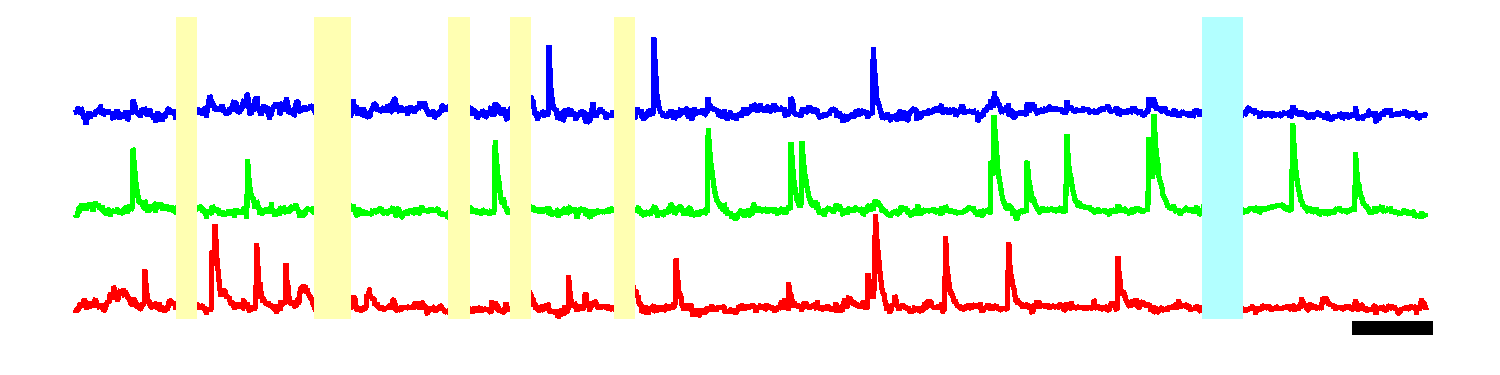
\includegraphics[height=0.8in,width=2.8in]{Fig_PFC_subfigs/example_temporal_cnmfe.pdf}}
\put(3.85, -6.7){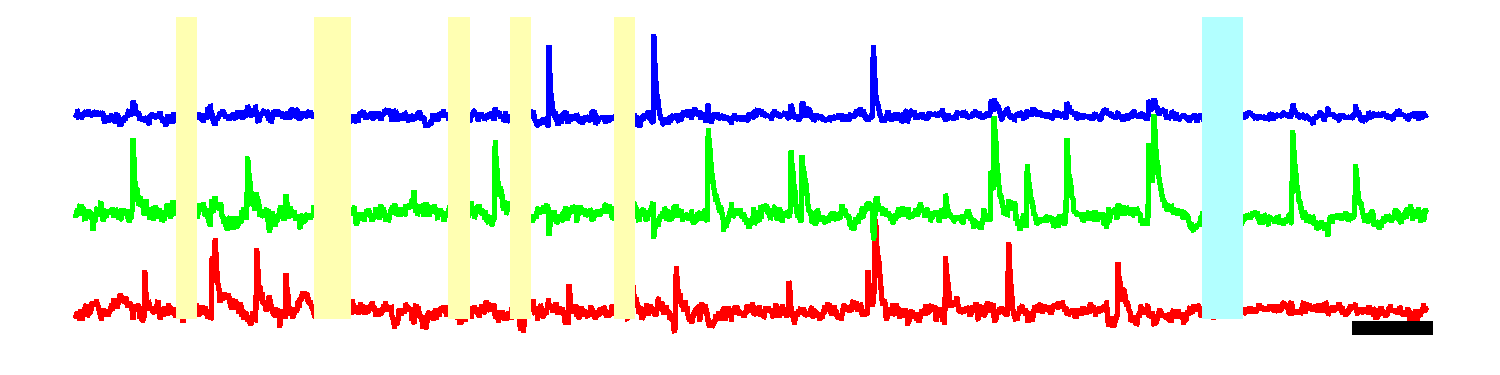
\includegraphics[height=0.8in, width=2.8in]{Fig_PFC_subfigs/example_temporal_ica.pdf}}

\put(3.3, -6.6){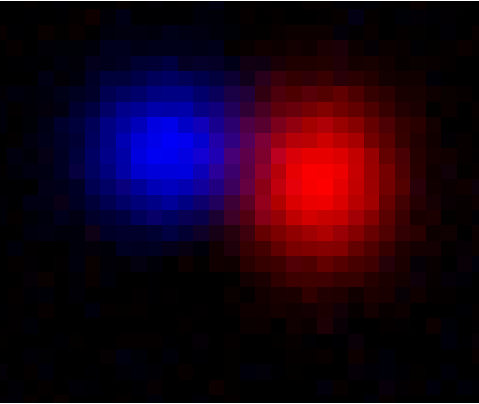
\includegraphics[height=0.6in]{Fig_PFC_subfigs/example_spatial_ica.pdf}}
\put(3.3, -5.9){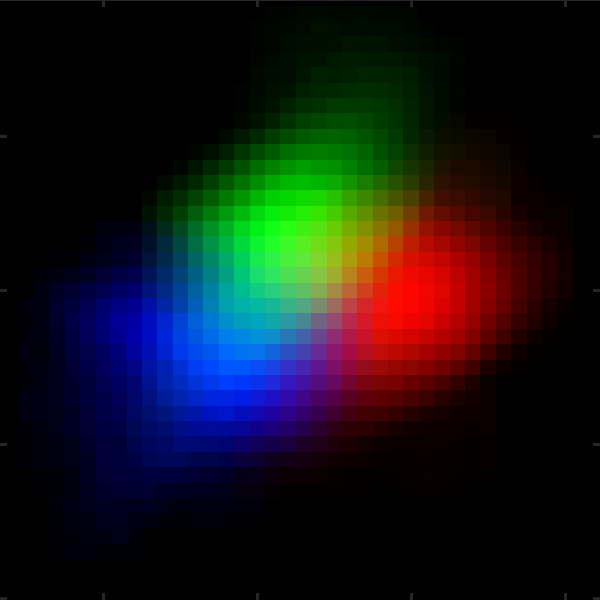
\includegraphics[height=0.6in]{Fig_PFC_subfigs/example_spatial_cnmfe.pdf}}
\put(3.15, -5.8){\rotatebox{90}{\scriptsize CNMF-E}}
% \put(3.12, -5.98){\line(1,0){3.5}}
% \put(3.12, -5.98){\line(0, 1){0.75}}
\put(3.12, -5.23){\large\textbf{G}}
\put(4.7, -5.18){\scriptsize Overlapping neurons}


\end{picture}
\end{document}
